% Created 2019-11-05 Tue 15:45
% Intended LaTeX compiler: pdflatex
\documentclass[11pt]{article}
\usepackage[utf8]{inputenc}
\usepackage[T1]{fontenc}
\usepackage{graphicx}
\usepackage{grffile}
\usepackage{longtable}
\usepackage{wrapfig}
\usepackage{rotating}
\usepackage[normalem]{ulem}
\usepackage{amsmath}
\usepackage{textcomp}
\usepackage{amssymb}
\usepackage{capt-of}
\usepackage{hyperref}
\graphicspath{ {./images/} }
\date{\today}
\title{}
\hypersetup{
 pdfauthor={},
 pdftitle={},
 pdfkeywords={},
 pdfsubject={},
 pdfcreator={Emacs 26.3 (Org mode 9.1.9)},
 pdflang={English}}
\begin{document}

%\tableofcontents

\section{Prediccion de clase de Iris Virginica e Iris Setosa haciendo uso de una red neuronal}
\label{sec:org62f021f}

\subsection{Introducción}
\label{sec:org9461112}
El objetivo de este trabajo es predecir correctamente la clase de un subgrupo (el 20\%) de flores iris con la menor cantidad de error posible, para esto se utilizo una red neuronal la cual fue entrenada con el 80\% de los datos. A continuación mostraremos los parámetros utilizados para conseguir un error de 10\(^{\text{-3}}\)

\subsection{Descripción de la base de datos}
\label{sec:orge27d66d}
La base de datos Iris contiene la variación morfológica de las 3 especies de flor, Iris Setosa, Iris Virginica e Iris Versicolor. La base datos de datos consiste de una colección de 50 flores y contiene información sobre 4 características:
Anchura del pétalo
Anchura del sépalo
Altura del pétalo
Altura del sépalo

\subsection{Red Neuronal}
\label{sec:orgc689a29}
\subsubsection{Función de activación}
\label{sec:orgb2a2ec9}
La red neuronal permite el uso de la función de umbral, la función lineal, lineal a trozos y la función sigmoide.
\subsubsection{Parámetros}
\label{sec:orga0bff03}
\begin{enumerate}
\item 3 Neuronas
\label{sec:org2c5c798}
Los parámetros utilizados fueron:
eta = 0.35
iteraciones = 15000
\begin{figure}[t]
    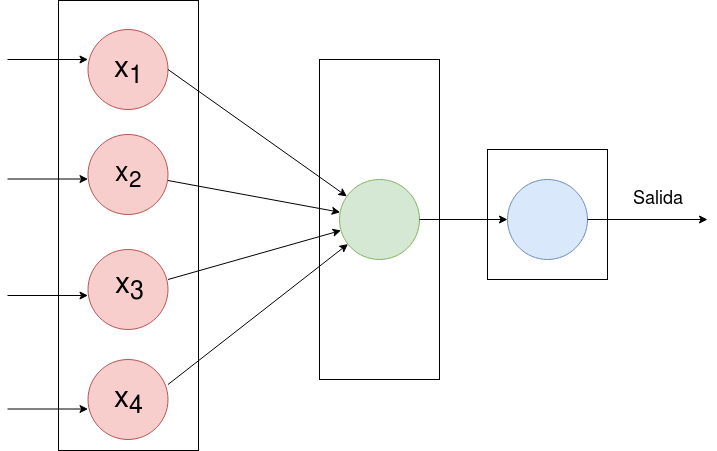
\includegraphics[width=10cm, height=10cm]{1hn}
    \centering
    \caption{}
    \label{1neurona}
\end{figure}

\begin{figure}[t]
    \includegraphics[width=10cm, height=10cm]{3Neu}
    \centering
    \caption{}
    \label{3neuronas}
\end{figure}


se encontró un error de 0.007 y se puede observar como alrededor de la iteraci\'on 200 se el error disminuye de manera considerable.
\end{enumerate}
\end{document}
